\subsection*{c. Obtener el nombre de todos los clientes que vivan en la región South y hayan solicitados productos de las subcategorías Bookcases o Chairs o Appliances o Copiers. El pedido debió de solicitarse el primer o tercer trimestre de 2015 y el modo de envío debe ser Standard Class.}

Renombramos las tablas \textit{customer}, \textit{orders} y \textit{products} como $c$, $o$ y $p$ respectivamente. Después realizamos un join entre $c$ y $o$ con el id del cliente, y al resultado le aplicamos otro join con $p$ con el id del producto, así cada fila tendrá la información del cliente, de la orden y del producto. \\ \\
Luego, proyectamos únicamente el nombre del cliente para obtener la lista de clientes que cumplen con todas las condiciones.

Expresión:
\[
\begin{aligned}
&\pi_{c.customername}\Bigg(
  \sigma_{\substack{
    c.region = \text{'South'} \;\\
    \land\; o.shipmode = \text{'Standard Class'} \; \\
    \land\;\big(\, (o.shipdate \geq \text{DATE('2015-01-01')} \;\land\; o.shipdate < \text{DATE('2015-04-01')}) \\
    \lor\; (o.shipdate > \text{DATE('2015-06-30')} \;\land\; o.shipdate < \text{DATE('2015-10-01')}) \,\big) \; \\
    \land\; \big(\, p.category = \text{'Bookcases'} \lor p.category = \text{'Chairs'} \\
                \lor\; p.category = \text{'Appliances'} \lor p.category = \text{'Copiers'} \,\big)
  }} \\
&\qquad\Big(
  \big( \rho_{c}(customer) \bowtie_{c.customerid = o.customerid} \rho_{o}(orders) \big)
  \bowtie_{o.productid = p.productid} \rho_{p}(products)
\Big)\Bigg)
\end{aligned}
\]
Resultados obtenidos:

\begin{figure}[h!]
\centering
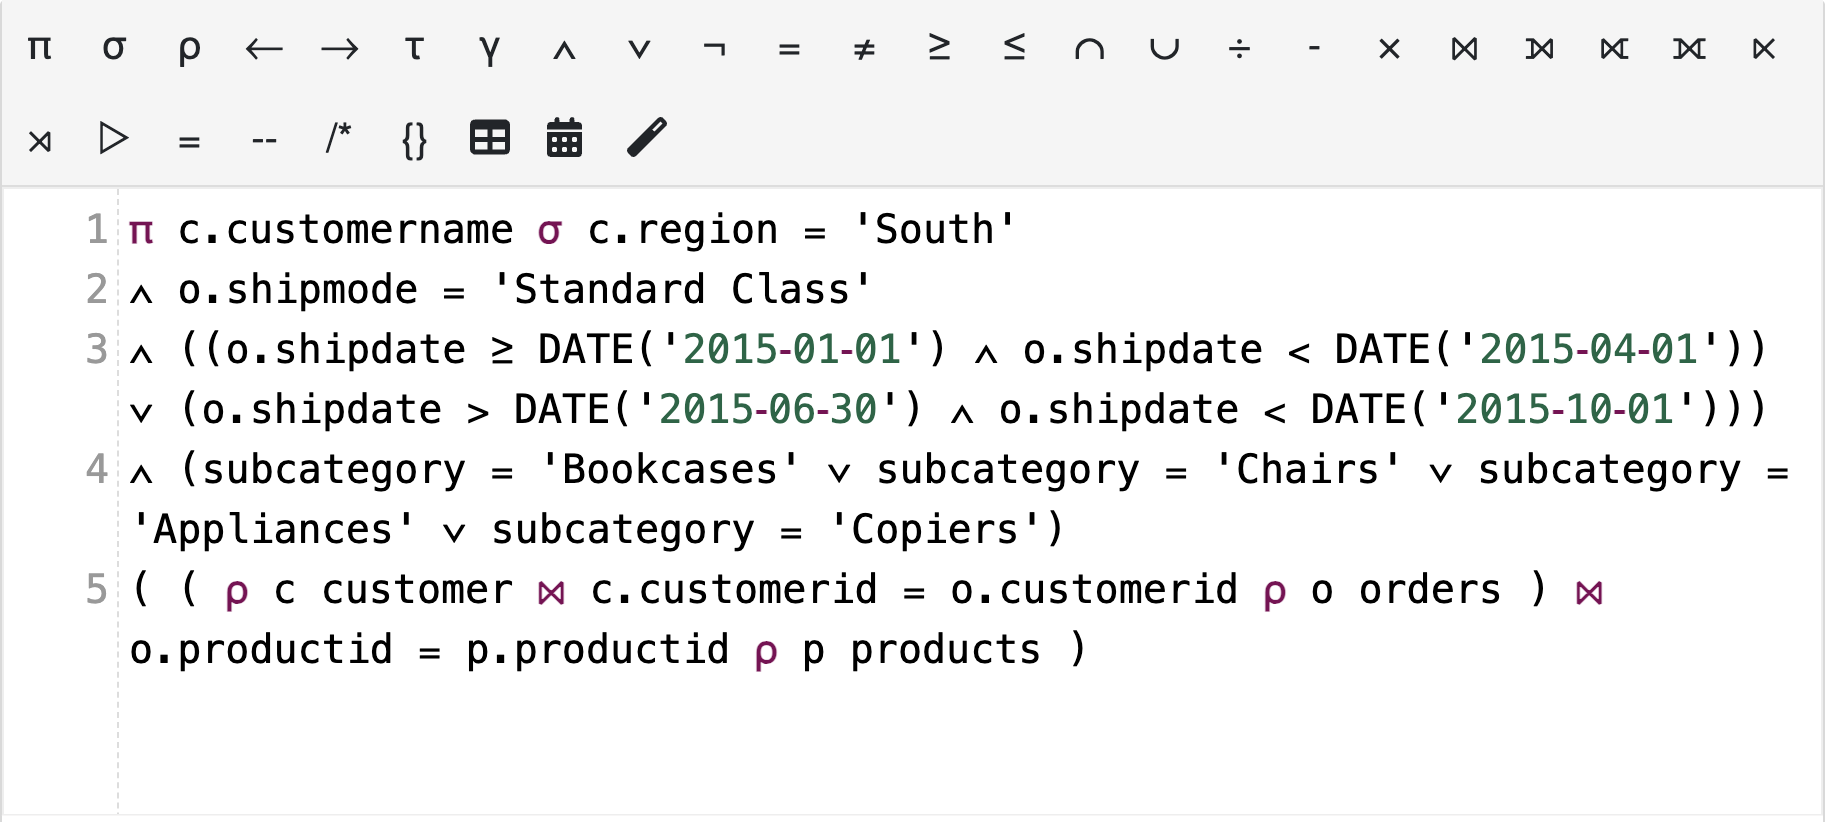
\includegraphics[width=0.8\textwidth]{imagenes/2c(1).png}
\caption{Consulta}
\end{figure}

\begin{figure}[h!]
\centering
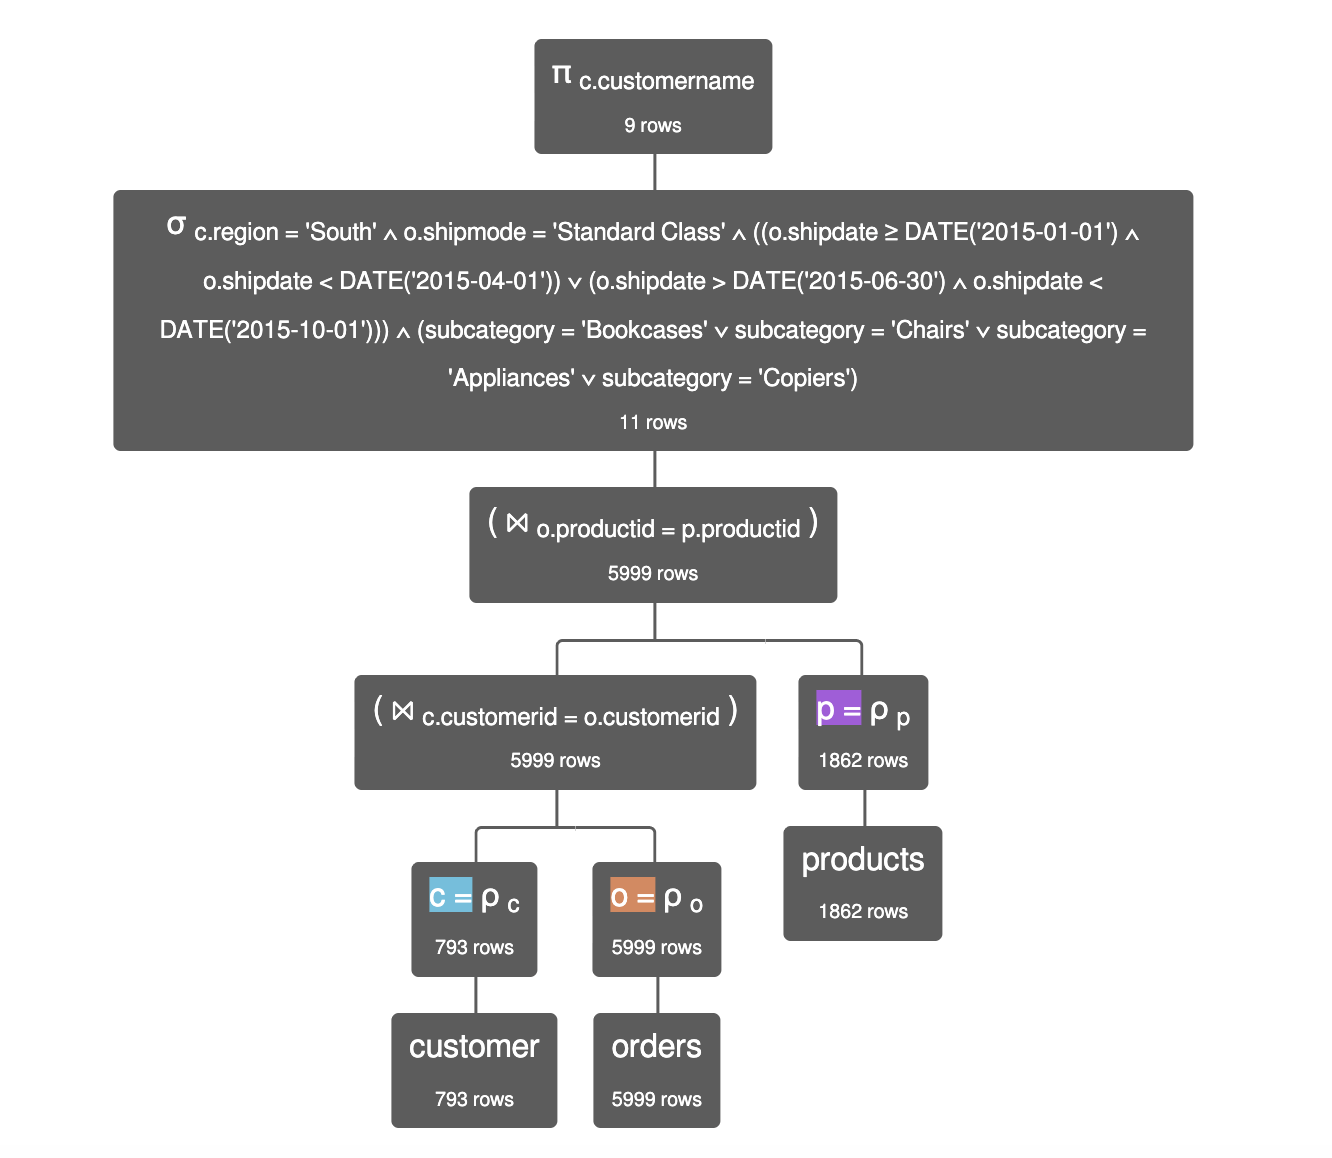
\includegraphics[width=0.8\textwidth]{imagenes/2c(2).png}
\caption{Árbol de consulta.}
\end{figure}

\begin{figure}[h!]
\centering
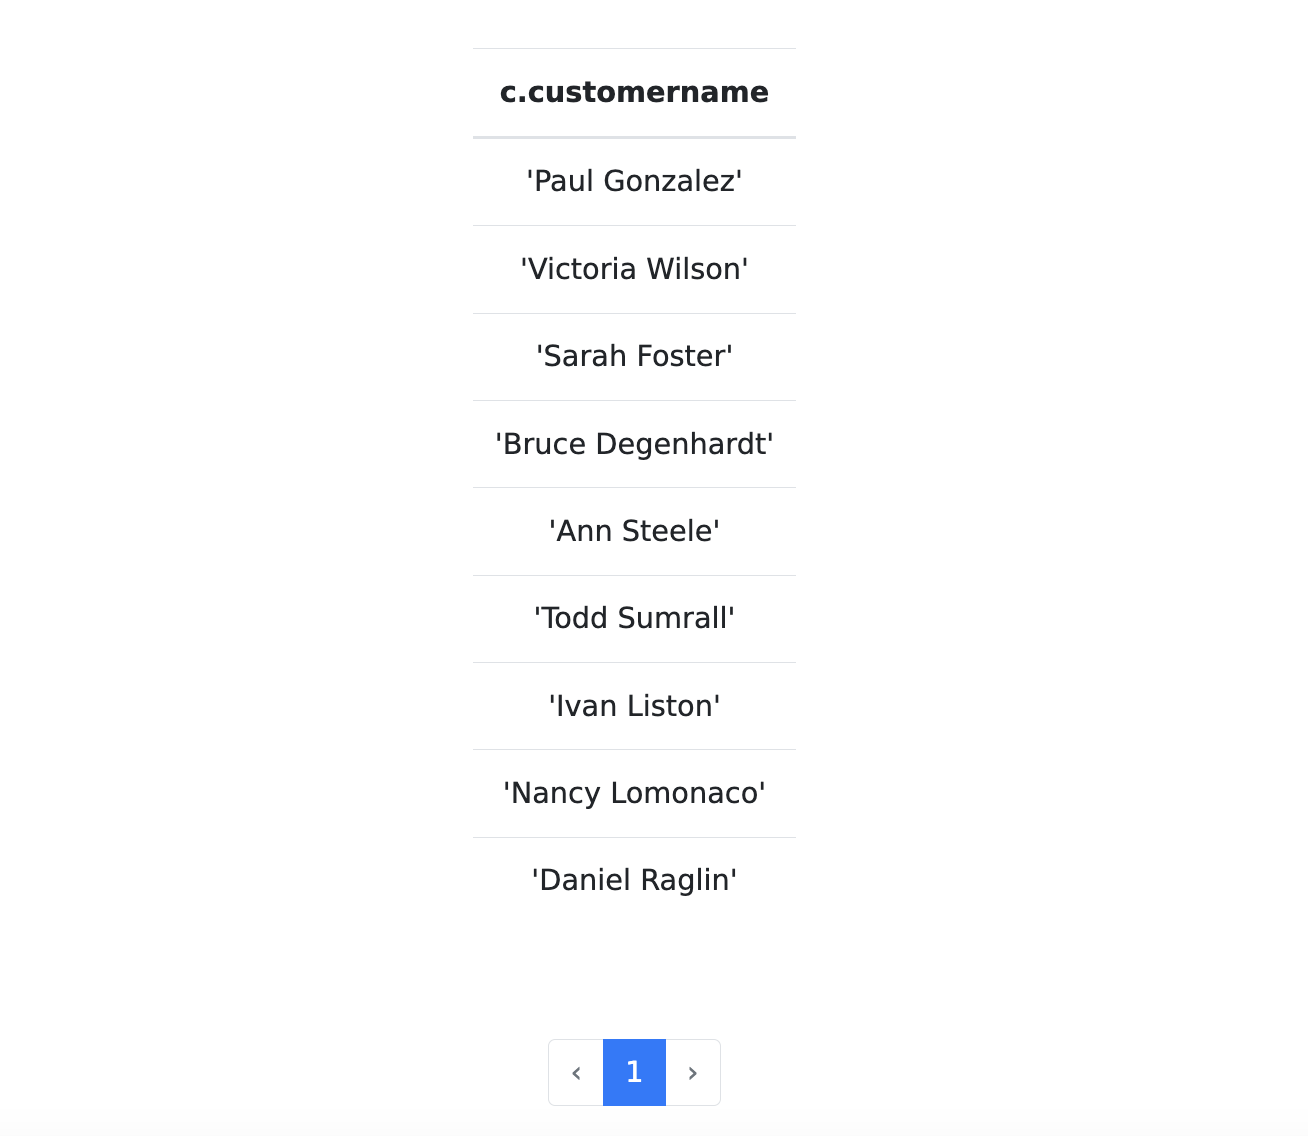
\includegraphics[width=0.6\textwidth]{imagenes/2c(3).png}
\caption{Resultado de consulta.}
\end{figure}
